\section{The Ainur Framework}\label{paper:olguinmunoz2022airnur:ainur}

\begin{figure}[t]
    \centering
    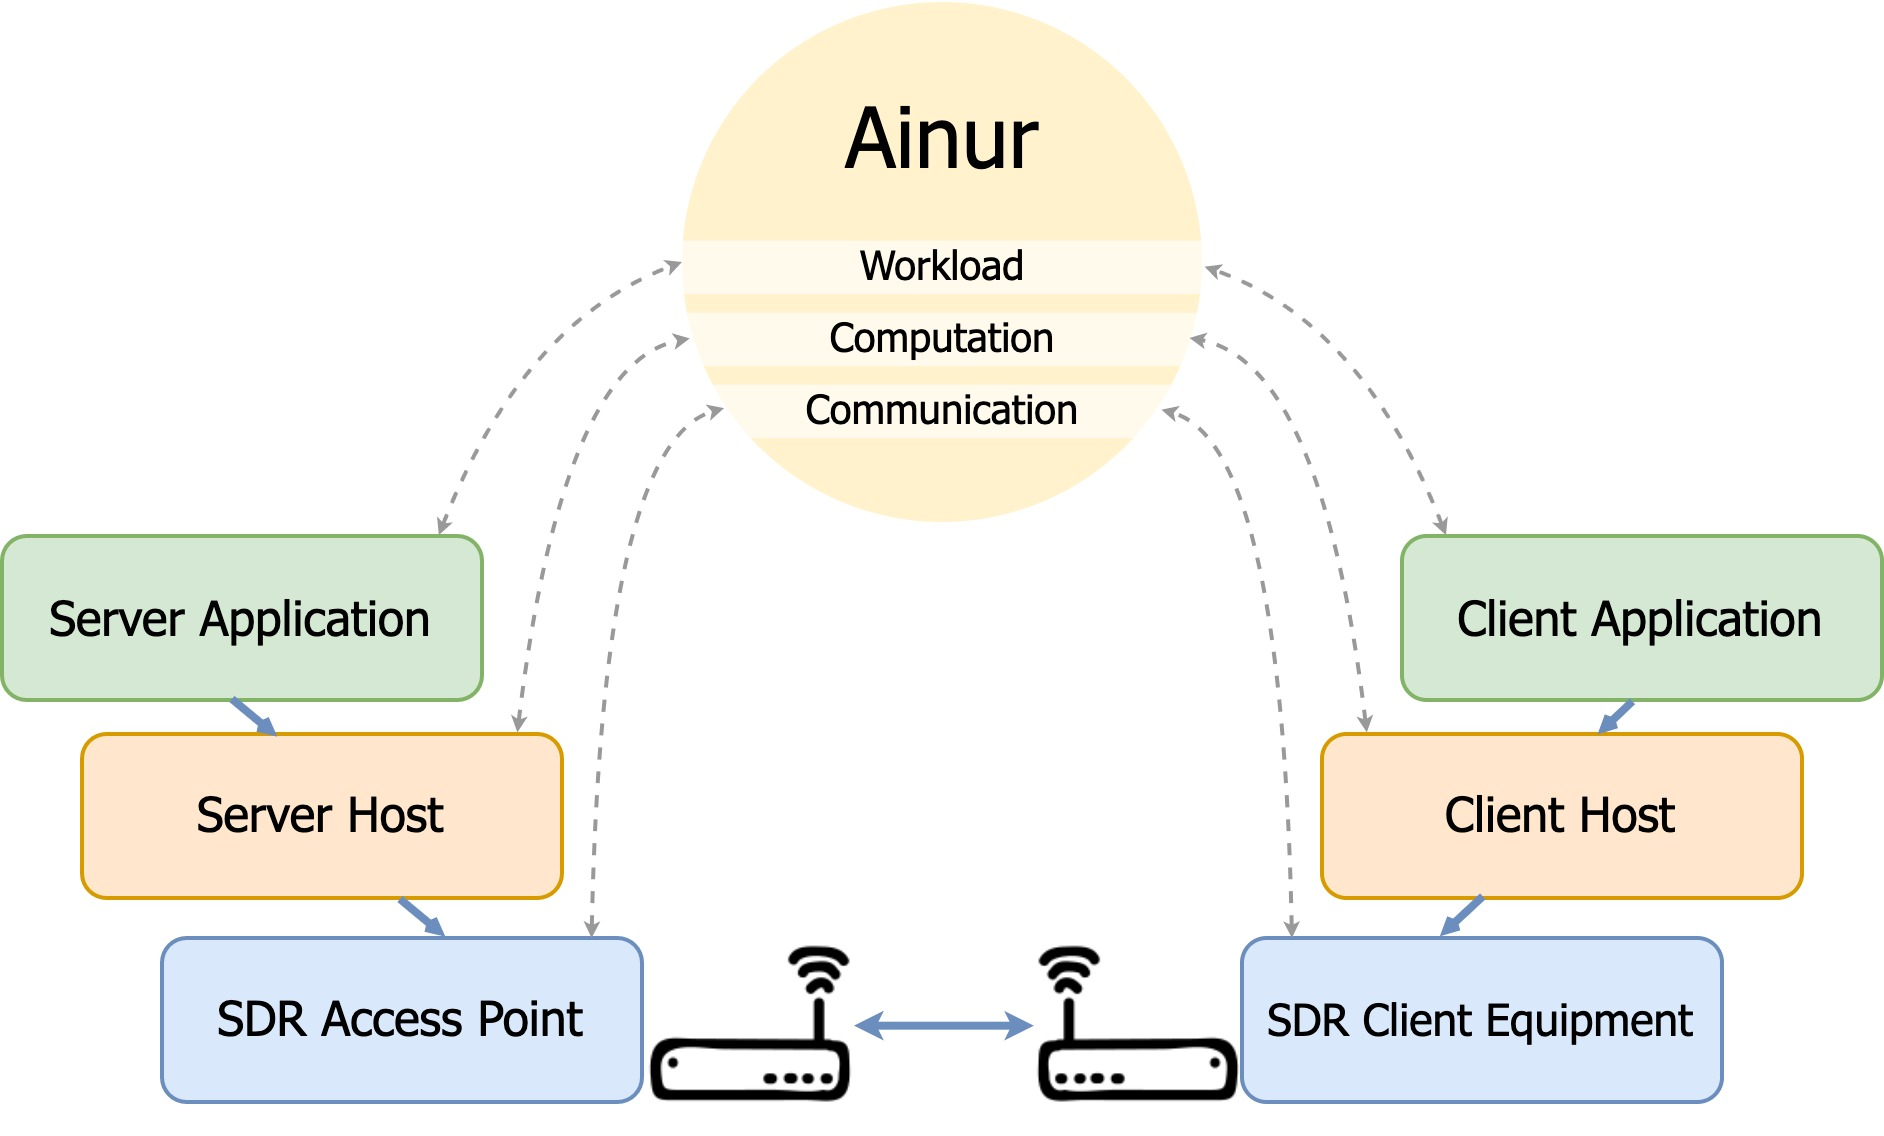
\includegraphics[width=\textwidth]{publications/2022Ainur/figures/overview}
    \caption{Layered structure of an Ainur experiment}\label{paper:olguinmunoz2022airnur:fig:overview}
\end{figure}

\begin{figure*}
    \centering
    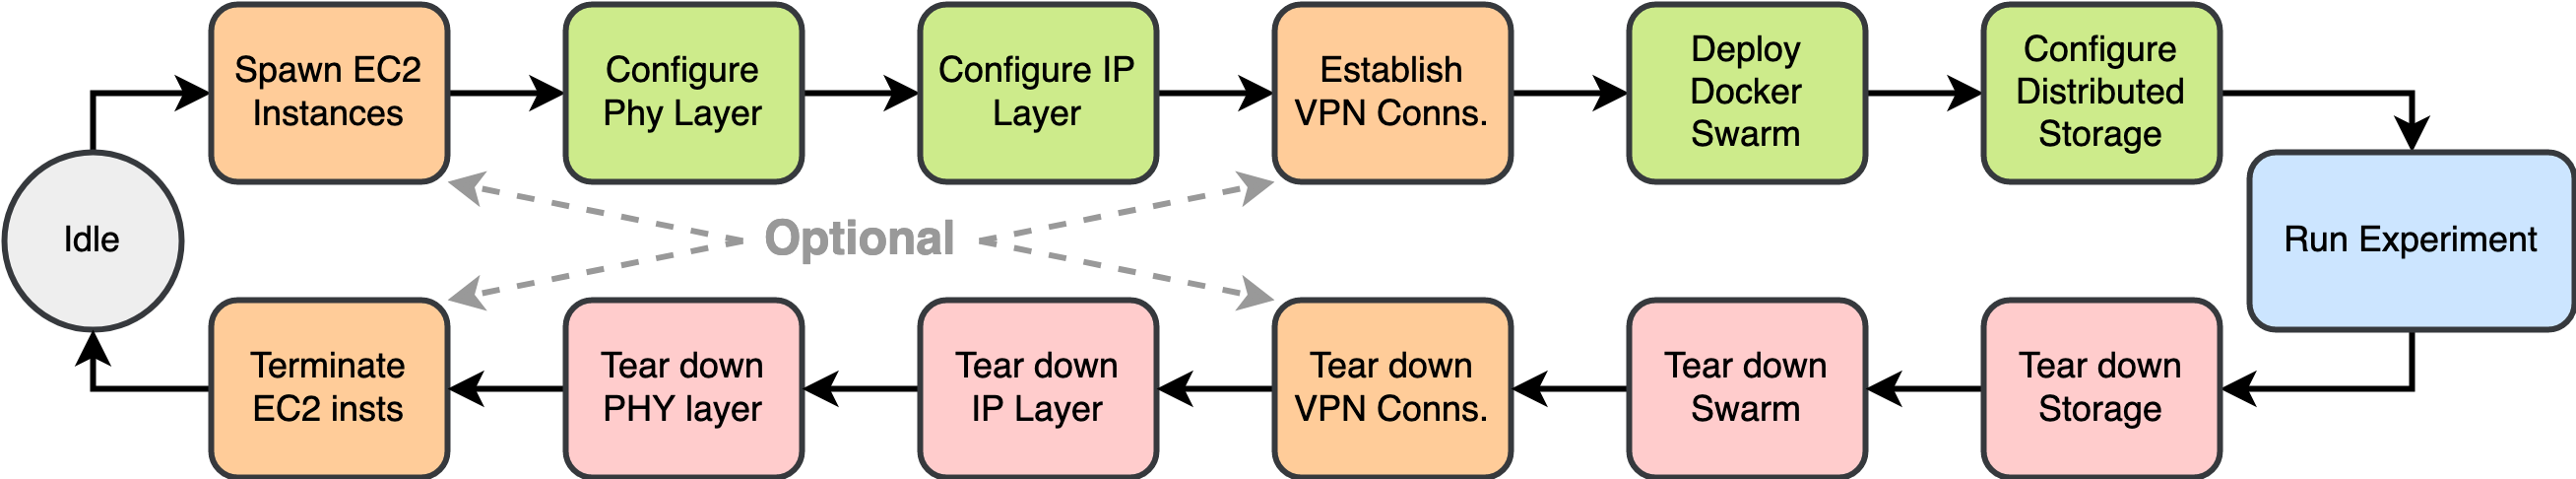
\includegraphics[width=\textwidth]{publications/2022Ainur/figures/flow2}
    \caption{Lifecycle of an experimental run in Ainur. Blocks in orange are optional.}\label{paper:olguinmunoz2022airnur:fig:flow}
\end{figure*}

\begin{figure*}
    \centering
    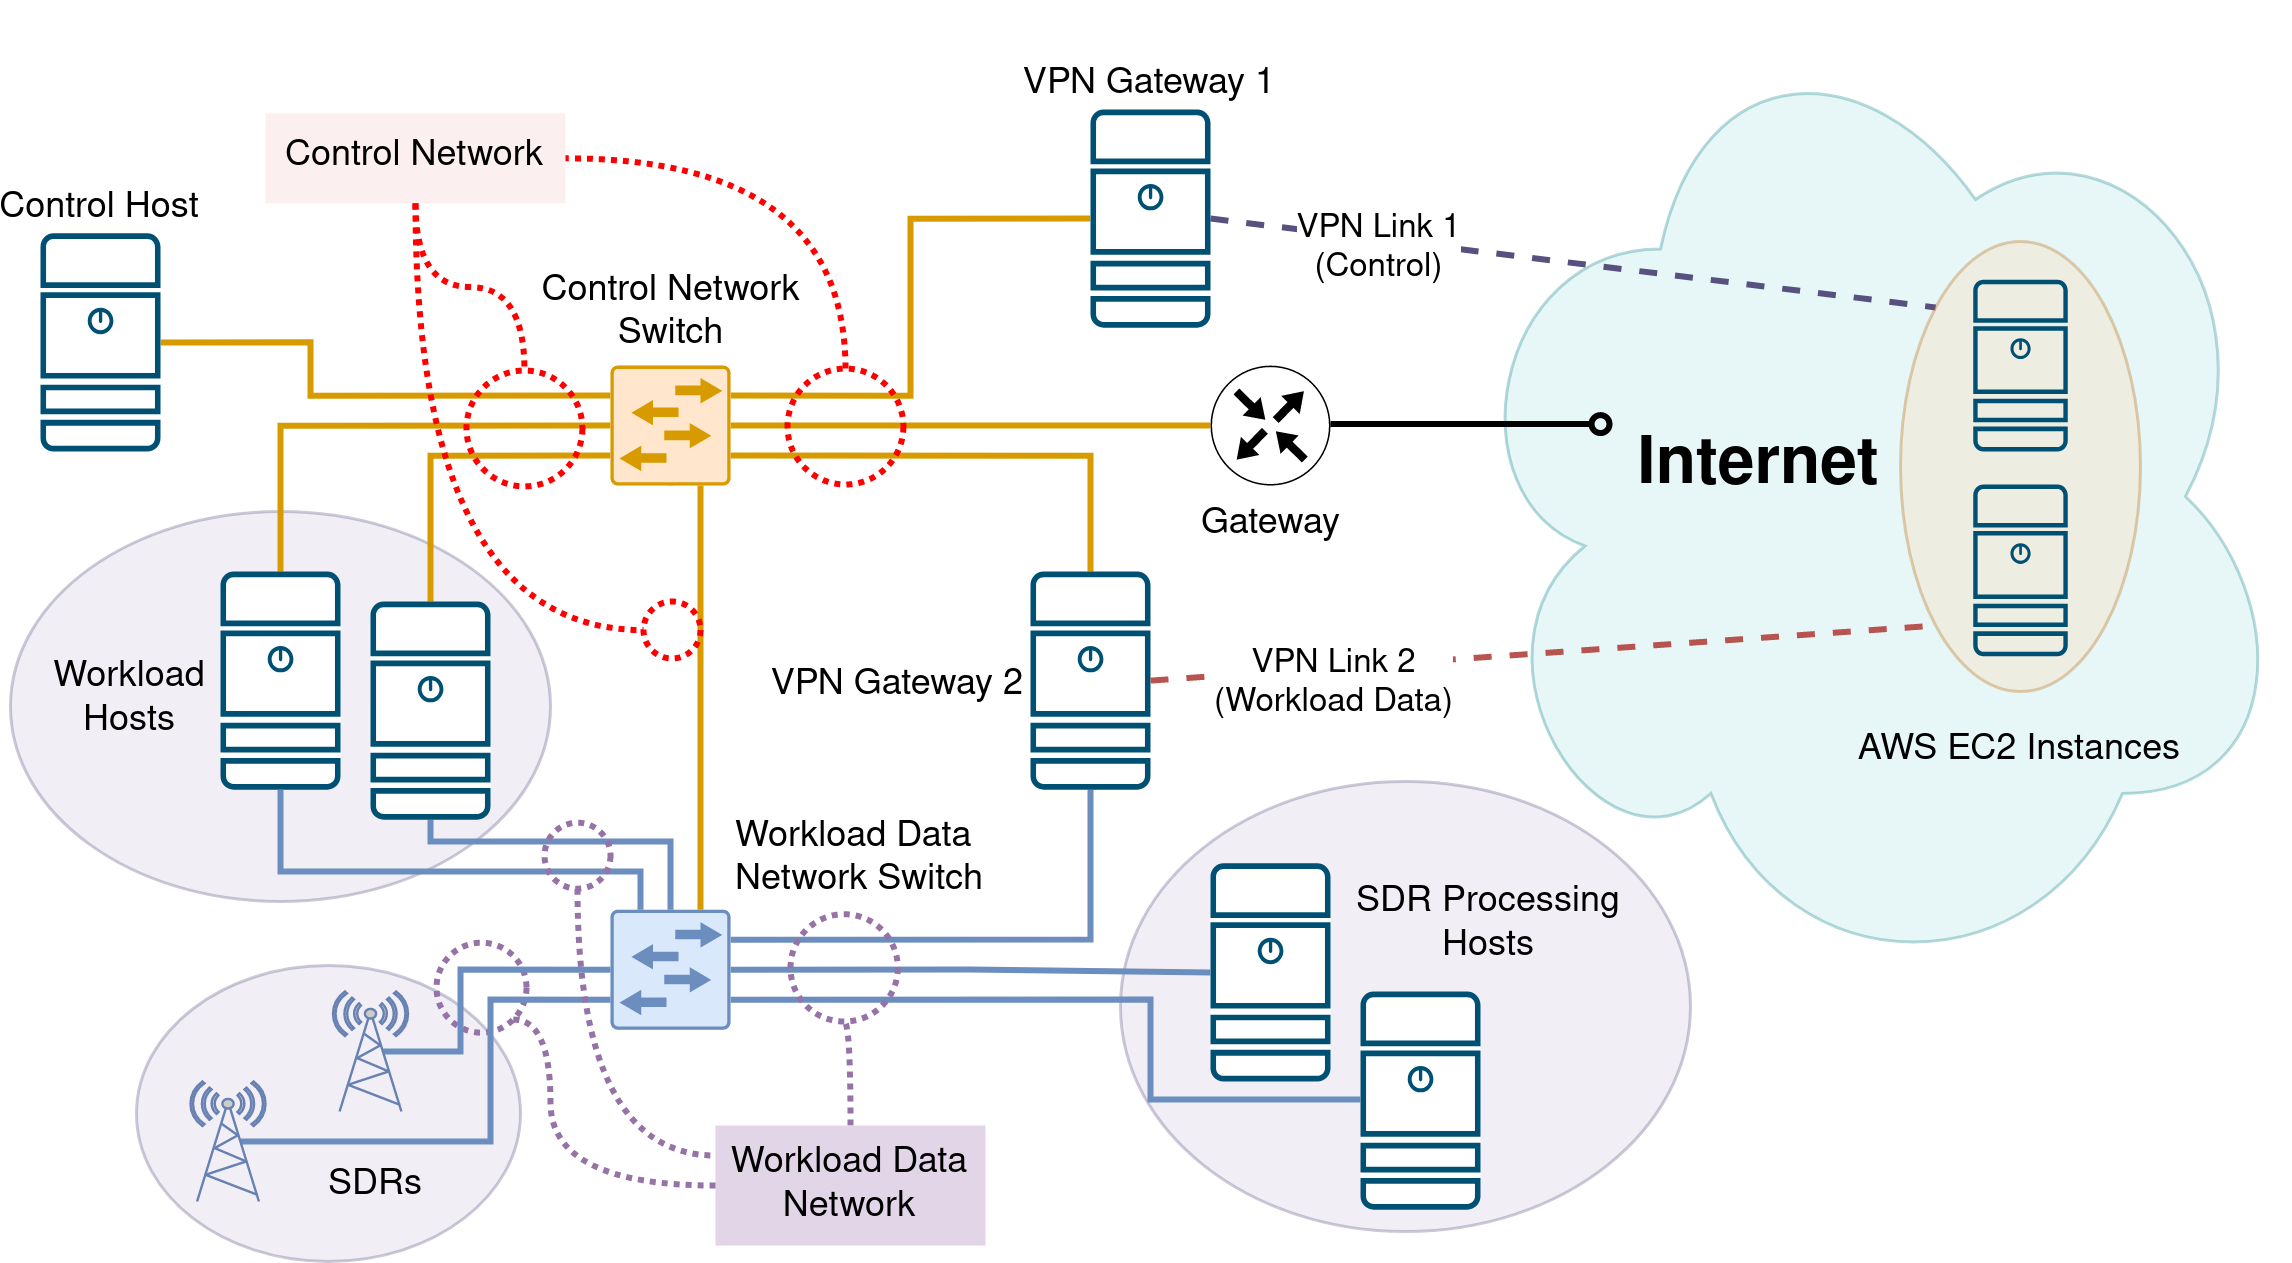
\includegraphics[width=\textwidth]{publications/2022Ainur/figures/network}
    \caption{Network structure assumed by Ainur.}\label{paper:olguinmunoz2022airnur:fig:network}
\end{figure*}

Ainur is designed as an end-to-end wireless network testbed management framework, fully flexible in terms of the communication network stack, computation hosts, and the distributed application deployed on top.
The core goal of the framework is to facilitate the creation of the desired communication and computation elements to discover their implications to the performance of end-to-end distributed applications.
Ainur achieves this by offering a Python \gls{API} which is used to describe an end-to-end experiment in a procedural manner, and we plan to eventually provide toolkits for declarative configuration of experiments.

Conceptually, in Ainur, an experiment is decomposed into a layered structure, consisting of
\begin{enumerate*}[itemjoin={{; }}, itemjoin*={{; and }}]
    \item the distributed application (workload)
    \item computation hosts
    \item communication networks connecting the hosts
\end{enumerate*}.
In \cref{paper:olguinmunoz2022airnur:fig:overview}, the workload is represented by a client-server process pair.
These could correspond, for instance, to the emulation of an inverted pendulum and a matching controller.
However, Ainur makes no assumptions about the nature of the workloads deployed on the framework, and virtually any process or combination of processes can be used.

Hosts correspond to either bare-metal machines or cloud instances on \gls{AWS} \gls{EC2}.
Users are free to combine and interconnect these in any configuration.
Ainur can provision wired networks over ethernet, and supports a number of software-defined wireless communication stacks, currently including Wi-Fi, 4G \gls{LTE}, and 5G.
To realize these various wireless communication protocols, it is assumed that the testbed is equipped with \gls{USRP} \gls{SDR}s and some computation hosts dedicated to signal processing and/or radio management.

To collect data from workloads, Ainur configures both a shared, distributed, storage location which all processes can reach, as well as a logging service which automatically captures structured and unstructured data from the standard output of workload processes.
The logging service additionally collects data from the other two layers, and the resulting dataset could, for instance, be analyzed to relate the performance of the control loop to the quality of the wireless link. 

\subsection{Ainur Software Stack}

To realize our vision for an automated, flexible, cloud-native, and workload-agnostic framework for cloud and edge computing experimentation, we built Ainur on top of a combination of well-established tools and frameworks.
Below we briefly touch on the most important of these:

\begin{description}
    \item[Python:]
    Ainur is built on-top of Python 3.8.
    We chose this language for its flexibility, ease of prototyping, and for the extensive ecosystem of third-party cloud-native frameworks and libraries.

    \item[Ansible:]
    One of the ``cloud-native frameworks'' mentioned above, Red Hat Ansible is a powerful Python framework for bare-metal configuration, provisioning, and automation.
    We use it extensively in Ainur for configuration of network interfaces and services on managed hosts.

    \item[Containers:]
    We leverage Docker containers to great extent for the virtualization and orchestration of workloads, as well as the encapsulation and management of complex network configurations.
    See \cref{paper:olguinmunoz2022airnur:containers} for more details.

    \item[\gls{AWS} and \texttt{boto3}:]
    Ainur employs the Amazon \texttt{boto3} library for Python to directly interface with \gls{AWS} \gls{EC2} and deploy, configure, and manage remote cloud instances.
    
    \item[\gls{OAI}:]
    \gls{OAI} is an open-source project that implements 3GPP technology on general purpose \texttt{x86} computing hardware and off-the-shelf \glspl{SDR} like the \gls{USRP}~\cite{kaltenberger2020openairinterface}.
    Ainur can deploy, configure, and manage \gls{OAI} software components that implement 4G \gls{LTE} and 5G \gls{NR}.
    
    \item[Mango Communications 802.11:]
    Finally, the Mango Communications project implements real-time 802.11 (Wi-Fi) MAC and PHY in Xilinx\\\glspl{FPGA}.
    It can be used on a variety of hardware platforms including \gls{USRP} \glspl{SDR}, and is employed in Ainur to provision end-to-end Wi-Fi links.
\end{description}

\subsection{Main Software Components}

Ainur follows a layered architecture which closely mimics the conceptual layers of the \gls{TCP}/\gls{IP} stack.
Components are deployed in bottom-up order, starting with the establishment of physical links, through the establishment of \gls{IP} connectivity and deployment of links to the cloud, and ending with the distribution and initialization of workloads on top of a container orchestration layer.
The architectural modules of the framework can broadly be classified according to the below categories:

\begin{description}[]
    \item[Configuration Layer:]
    The lowest layer of Ainur.
    It handles the parsing of configuration files describing experimental scenarios.
    Optional, as it is only needed when Ainur is running experiments described in a declarative manner.

    \item[Logging layer:]
    This layer handles logging across all layers of the system to a central repository.
    Concretely, it manages the configuration and lifecycle of a Fluentd server to which any component in the network can send logs.
    Currently, the two main components relying on this scaffolding are the physical layer and the workloads.
    
    \item[Physical Layer:] 
    Creates and deploys the underlying physical connections of the workload data network.
    This layer interacts with hardware such as managed switches and \glspl{SDR} (and their associated computation hosts) to create links between the desired workload hosts.
    These links correspond to ethernet, Wi-Fi, and even an entire software-defined 4G \gls{LTE} and 5G networks.

    \item[Cloud Layer:]
    Handles integration with cloud services (currently, \gls{AWS} \gls{EC2}).
    Only deployed in the case of an experiment requiring cloud instances, it manages the instantiation and configuration of remote cloud resources.

    \item[\gls{IP} Layer:]
    Configures and establishes \gls{IP} layer connectivity of packets between hosts in the experimental setup, both local and cloud.
    This includes assigning valid \gls{IP} addresses to hosts, establishing \gls{VPN} routes to cloud instances through a pair of pre-configured \gls{VPN} gateways, and configuring routing tables to ensure any two hosts in the workload network can communicate with each other.

    \item[Workload Layer:]
    Finally, this layer deploys, scales, and orchestrates containerized workloads, as well as configures a shared, distributed storage for workloads to store data.
    This components leverages Docker Swarm to spin up and manage workload containers on desired hosts.
    It also establishes overlay networks abstracting away the physical topology and allowing containers to interconnect through dynamically assigned hostnames.
\end{description}

\subsection{Containerization}\label{paper:olguinmunoz2022airnur:containers}

Containers are a key cloud-native technology for the virtualization and sandboxing of arbitrary processes~\cite{merkel2014docker}.
They allow for easy packaging of software in predefined, consistent, and conflict-free execution environments, including all necessary dependencies.
Containers are lightweight and portable compared to \gls{VM}-based virtualization, making them an ideal solution for the distribution, deployment, and orchestration of software in distributed computing environments.
They deploy quickly and are very configurable, while abstracting away the complexities and delays that come with in creating, managing, and moving (potentially huge) \gls{VM} disk images.

Ainur leverages containerization extensively across the framework, in order to
\begin{enumerate*}[itemjoin={{, }}, itemjoin*={{, and }}]
    \item deploy and orchestrate workloads
    \item support a wide spectrum of different physical layer configurations out-of-the-box, as well as allow for easy extension to new ones
    \item support automated collection of logs
\end{enumerate*}.
Workloads in the framework are deployed packaged in Docker containers, orchestrated through \texttt{docker-compose} and Docker Swarm.
We have selected Docker Swarm as our container orchestration layer instead of more advanced toolkits such as Kubernetes due to
\begin{enumerate*}[itemjoin={{; }}, itemjoin*={{; and }}]
    \item it being more lightweight
    \item its comparative simplicity in terms of configuration and setup
    \item the fact that it is included in the default Docker runtime installation
\end{enumerate*}.
This allows the framework to remain mostly agnostic to the nature of the workloads, and thus support a wide ranged of different applications and system architectures.
It also allows for easy deployment to different compute nodes in the network, without having to take into consideration details such as required libraries and versions.

As expressed above, Ainur also leverages containers for the communication stack.
With the advent of \gls{O-RAN} and \glspl{SDR}, all components of the wireless network stack can run on general-purpose processors.
They can thus be containerized and distributed across multiple hosts.

As a final point, the automation of logging is another advantage of using containers and an orchestration framework.
Ainur employs the Fluentd unified layer for log collection.
It natively integrates with Docker containers and allows for the automatic collection of text data from the standard output and error streams of processes executing inside containers.
It automatically decouples data sources from containers running on different systems and allows Ainur to collect and classify the logs from any components of the network, whether on the wireless stack or workload.

\subsection{Obtaining Ainur and deploying it on a new testbed}

\begin{figure}
    \centering
    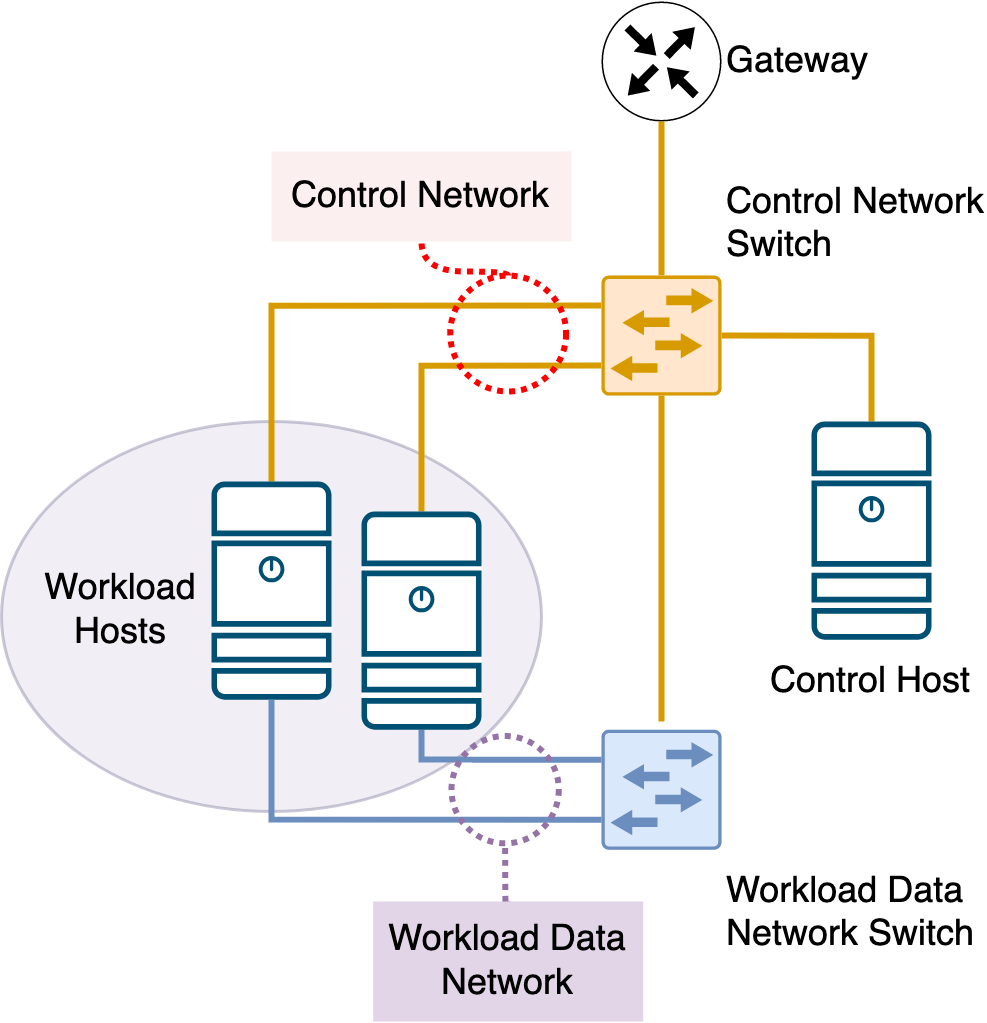
\includegraphics[height=25em]{publications/2022Ainur/figures/network-minimal}
    \caption{Minimal testbed setup on which Ainur can be deployed.}\label{paper:olguinmunoz2022airnur:fig:network:minimal}
\end{figure}

The framework is released as \gls{FOSS} under a permissive Apache license.
It can be downloaded from the Ainur repository~\cite{ainur:github} of the {KTH-EXPECA} organization on GitHub.
Given the software's complexity, the repository also includes detailed documentation on its requirements, configuration, deployment, and execution, as well as links to external resources containing information and guides about related concepts and services.

Ainur makes a number of assumptions about its execution environment.
Apart from generic ones regarding the presence of necessary authentication information for remote access to local and remote hosts and services, the framework assumes a split network architecture.
Ainur runs in a dedicated control host and the management plane resides in a physically distinct network from the workload data.
This is a key requirement to be able to reconfigure the physical links in the workload data network without disrupting management traffic.

A full-featured, and rather complex deployment is depicted in \cref{paper:olguinmunoz2022airnur:fig:network}, including a number of optional testbed features such as offload to the cloud through \gls{VPN} gateways.
However, a minimal a setup can be achieved with a control host, at least two workload hosts, and a couple of managed (smart) switches, as illustrated in \cref{paper:olguinmunoz2022airnur:fig:network:minimal}.
The only requirements for the aforementioned hosts are that a general purpose Linux distribution such as Ubuntu can be deployed on them, and --- in the case of the workload hosts --- the presence of two network interfaces.
Thus, a minimal testbed can be achieved cheaply and quickly by employing small single-board computers such as Raspberry Pi, Jetson Nano, or BeagleBone units.
Finally, the configuration and deployment of an Ainur-compatible testbed can be easily automated with tools such as Ansible, and playbooks for this effect can be made available to the community upon request.

% Also assumed is the existence of \gls{VPN} gateways to the cloud, time synchronization, and configured hostname lookups (possibly using a \gls{DNS} service).
